\documentclass[border=2pt]{standalone}
\usepackage{tikz}
\usepackage{amsmath}
\usepackage{bm}
\usetikzlibrary{positioning, shapes.geometric}
\usetikzlibrary{decorations.pathreplacing}

\definecolor{darkred}{rgb}{0.9, 0, 0}

\begin{document}
    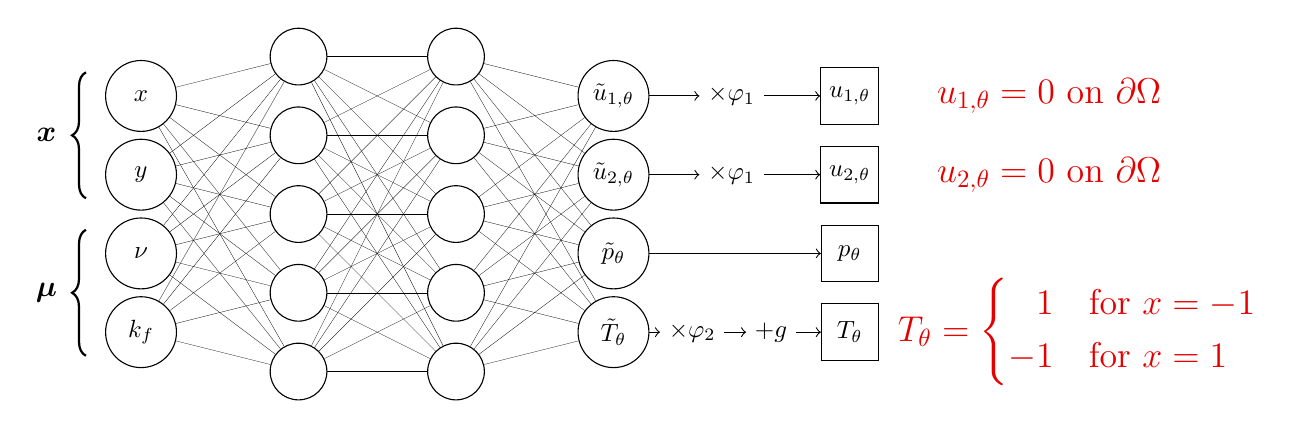
\begin{tikzpicture}[%circle red
        neuron/.style={circle, draw, minimum size=0.8cm},
        inout/.style={circle, draw, minimum size=1cm},
        %other circle with no border
        final/.style={rectangle, draw, minimum size=0.8cm},
        label/.style={font=\footnotesize},
        every node/.style={scale=0.9}
    ]

    % Entrées
    \foreach \i/\name in {1/x,2/y,3/{\nu},4/{k_f}} {
        \node[inout] (in\i) at (0,-0.5-\i) {$\name$};
        }
        
    % Accolade pour x et y
    \draw[decorate, decoration={brace, amplitude=5pt}, thick]
    (-0.7,-2.8) -- (-0.7,-1.2);
    \node at (-1.2,-2) {\large $\bm{x}$};

    % Accolade pour mu et kf
    \draw[decorate, decoration={brace, amplitude=5pt}, thick]
    (-0.7,-4.8) -- (-0.7,-3.2);
    \node at (-1.2,-4) {\large $\bm{\mu}$};
        
    % Couches fully connected : 2 couches de 5 neurones
    \foreach \layer/\x in {1/2, 2/4} {
        \foreach \i in {1,...,5} {
            \node[neuron] (h\layer\i) at (\x,-\i) {};
        }
    }
            
    % Sorties tilde
    \foreach \i/\name in {1/{\tilde{u}_{1,\theta}}, 2/{\tilde{u}_{2,\theta}}, 3/{\tilde{p}_\theta}, 4/{\tilde{T}_\theta}} {
        \node[inout] (out\i) at (6,-0.5-\i) {$\name$};
    }
    
    % Connexions fully connected
    \foreach \i in {1,...,4} {
        \foreach \j in {1,...,5} {
            \draw[-, ultra thin] (in\i) -- (h1\j);
        }
    }
    \foreach \i in {1,...,5} {
        \foreach \j in {1,...,5} {
            \draw[-, ultra thin] (h1\i) -- (h2\j);
        }
    }
    \foreach \i in {1,...,5} {
        \foreach \j in {1,...,4} {
            \draw[-, ultra thin] (h2\i) -- (out\j);
        }
    }            

    % Post-processing
    \node (mult1) at (7.5,-1.5) {$\times\varphi_1$};
    \draw[->] (out1) -- (mult1);
    \node[final] (f1) at (9,-1.5) {$u_{1,\theta}$};
    \draw[->] (mult1) -- (f1);

    \node (mult2) at (7.5,-2.5) {$\times\varphi_1$};
    \draw[->] (out2) -- (mult2);
    \node[final] (f2) at (9,-2.5) {$u_{2,\theta}$};
    \draw[->] (mult2) -- (f2);

    \node[final] (f3) at (9,-3.5) {$p_\theta$};
    \draw[->] (out3) -- (f3);

    \node (mult4) at (7,-4.5) {$\times\varphi_2$};
    \draw[->] (out4) -- (mult4);
    \node (mult4b) at (8,-4.5) {$+g$};
    \draw[->] (mult4) -- (mult4b);
    \node[final] (f4) at (9,-4.5) {$T_\theta$};
    \draw[->] (mult4b) -- (f4);

    % BC
    \node[anchor=west] at (10,-1.5) {\textcolor{darkred}{\Large $u_{1,\theta}=0$ on $\partial\Omega$}};
    \node[anchor=west] at (10,-2.5) {\textcolor{darkred}{\Large $u_{2,\theta}=0$ on $\partial\Omega$}};

    \node[anchor=west, align=center] at (9.5,-4.5) {\Large \textcolor{darkred}{$T_\theta=\left\{
        \begin{aligned}
            &1 \quad \text{for } x=-1 \\
            -&1 \quad \text{for } x=1
        \end{aligned}
    \right. $}};

    \end{tikzpicture}
\end{document}
